\subsection{Test Flashed Sample}

Open a serial terminal with e.g. PuTTY to see the log output.

\begin{monobox}
plink -sercfg 115200 -serial com3
\end{monobox}

The output should look like this:

\begin{lstlisting}
*** Booting Zephyr OS build zephyr-v@\zephyrversion{}@ ***
...
\end{lstlisting}

You might have to press the reset button on your microcontroller board to start the program and print the message again.

\begin{infobox}
  Open the device manager to find the COM-port number.
  \begin{center}
    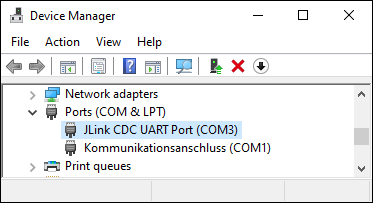
\includegraphics[width=.5\paperwidth]{device_manager_com}
  \end{center}
\end{infobox}
